\documentclass[tikz]{standalone}

\usepackage{euler}

\usepackage[compat=1.1.0]{tikz-feynman}
\tikzset{cross/.style={cross out, draw=black, minimum size=2*(#1-\pgflinewidth), inner sep=0pt, outer sep=0pt},
%default radius will be 1pt. 
cross/.default={1pt}}

\begin{document}

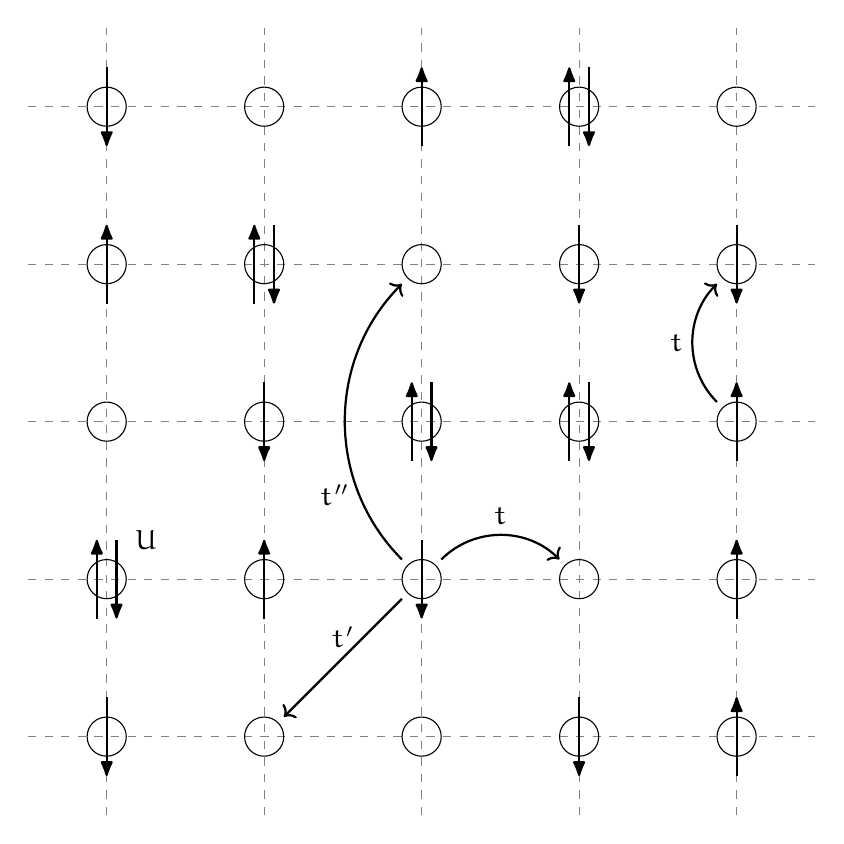
\begin{tikzpicture}
    \draw[style=help lines,dashed] (-5,-5) grid[step=2cm] (5,5);
    \foreach \x in {-2,-1,...,2}{
        \foreach \y in {-2,-1,...,2}{
            \node[draw,circle,inner sep=5pt] at (2*\x,2*\y) {};
      }
    }
    % 1st row
    \draw[{Latex[round]-}, thick] (-4, 3.5) -- (-4, 4.5);
    \draw[-{Latex[round]}, thick] (0, 3.5) -- (0, 4.5);
    \draw[-{Latex[round]}, thick] (1.875, 3.5) -- (1.875, 4.5);
    \draw[{Latex[round]-}, thick] (2.125, 3.5) -- (2.125, 4.5);
    
    % 2nd row
    \draw[-{Latex[round]}, thick] (-4, 1.5) -- (-4, 2.5);
    \draw[-{Latex[round]}, thick] (-2.125, 1.5) -- (-2.125, 2.5);
    \draw[{Latex[round]-}, thick] (-1.875, 1.5) -- (-1.875, 2.5);
    \draw[{Latex[round]-}, thick] (2, 1.5) -- (2, 2.5);
    \draw[{Latex[round]-}, thick] (4, 1.5) -- (4, 2.5);
    
    % 3rd row
    \draw[{Latex[round]-}, thick] (-2, -0.5) -- (-2, 0.5);
    \draw[-{Latex[round]}, thick] (-0.125,-0.5) -- (-0.125,0.5);
    \draw[{Latex[round]-}, thick] (0.125,-0.5) -- (0.125,0.5);
    \draw[-{Latex[round]}, thick] (1.875,-0.5) -- (1.875,0.5);
    \draw[{Latex[round]-}, thick] (2.125,-0.5) -- (2.125,0.5);
    \draw[-{Latex[round]}, thick] (4,-0.5) -- (4,0.5);
    
    % 4th row
    \draw[-{Latex[round]}, thick] (-4.125,-2.5) -- (-4.125,-1.5);
    \draw[{Latex[round]-}, thick] (-3.875,-2.5) -- (-3.875,-1.5);
    \draw[-{Latex[round]}, thick] (-2,-2.5) -- (-2,-1.5);
    \draw[{Latex[round]-}, thick] (0,-2.5) -- (0,-1.5);
    \draw[-{Latex[round]}, thick] (4,-2.5) -- (4,-1.5);
    
    % 5th row
    \draw[{Latex[round]-}, thick] (-4,-4.5) -- (-4,-3.5);
    \draw[{Latex[round]-}, thick] (2,-4.5) -- (2,-3.5);
    \draw[-{Latex[round]}, thick] (4,-4.5) -- (4,-3.5);
    
    % hopping
    \draw[->, thick] (0.25,-1.75) to [bend left=45] node[midway, above] {$t$} (1.75,-1.75);
    \draw[->, thick] (-0.25,-2.25) to node[midway, above] {$t'$} (-1.75,-3.75);
    \draw[->, thick] (-0.25,-1.75) to [bend left=45] node[near start, left] {$t''$} (-0.25,1.75);
    \draw[->, thick] (3.75, 0.25) to [bend left=45] node[midway, left] {$t$} (3.75,1.75);
    
    % interaction U
    \node at (-3.5, -1.5) {$U$};
\end{tikzpicture}

\end{document}
